\thispagestyle{fancy}
\chapter{Continous Integration}
\label{chp:contintegration}

\section{Versionstyring}
Versionsstyringsværktøjet Git og tilhørende Git server gjorde det muligt, for hvert gruppemedlem at arbejde individuelt med en del af opgaven. Ved afsluttet delopgave blev dette tilføjet til det samlede projekt på Git serveren. De andre gruppemedlemmer skulle pulle og merge deres arbejde med den nyeste udgave a projektet inden deres eget arbejde kunne pushes til serveren. Der kunne til tider opstå merge conficts hvilket resulterede i lidt ekstra arbejde, men da versionsstyring og mergetools er tilgængelig blev disse problemer let løst. Selv om det er muligt, at arbejde på separate brances blev dette ikke særlig aktuelt, da de enkelte arbejdsopgaver ikke var bredtfavnende.   

\section{Buildserver}
Jenkins er benyttet som buildserver til at udelukke alle lokale indspillende faktorer ved compiling af projektet. Jenkins er linket op mod gruppens Git repository og bygger den seneste udgave af projektet hver gang der pushes til branchen master. Efter projektet er blevet bygget af Jenkins rapporterers der tilbage om projektet kunne compiles eller ej. Udfaldet bliver lagt i en byggehistorik, hvor det også er muligt at se detaljer om tidligere byg. Alle medlemmer af gruppen fik garanteret, at deres tilføjelser til det samlede projekt ikke spolerede udviklingsarbejdet hos de andre i gruppen når der skulle pulles og merges. Endvidere gjorde to plugins til DotCover og NUnit det muligt, at se om alle tests og codecoverage var som forventet.

\subsection{DotCover}
Dot cover er en statisk kodeanalyse værktøj der analyserer hvor mange linjer kode vi tester.  Det er muligt at ekskludere code der ikke skal tages med i analysen. Det kan være klasser, moduler eller funktioner. Vi har besluttet at code coveres skal være 100 \%, det betyder dog ikke at vi kan være sikre på at kodens funktionalitet er testet, men blot at alle linjer kode har været berørt af vores unit test. Det vil sige at det ikke er funktionaliteten der er testet.

\subsection{NUnit}
NUnit er et open source testing framework for udvikling af projekter i .Net. Alle unittests er baseret på NUnit konventioner og gruppen benyttede sig af dette til at teste klasser og underliggende metoder. Disse tests blev også eksekveret på Jenkis serveren, og resultatet der fra vist på projektets forside.

\begin{figure}[h!]
	\centering
		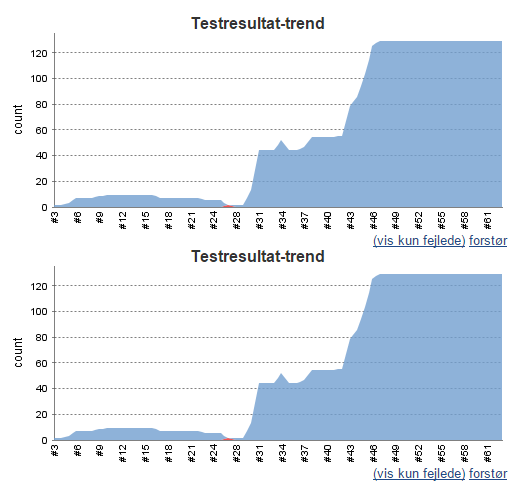
\includegraphics[width=0.8\textwidth]{NUnit_test_results}}
	\caption{NUnit testresultater fra Jenkins.}
\end{figure}

%\section{Strategi}
%Fra start var gruppen enig om at dele sig ud i 2 par og arbejde i pair programming. På den måde kunne der arbejdes på to dele af designet på en gang. Kvaliteten blev dermed højnet af at der var fire øjne på skærmen, mens der blev programmeret og taget beslutninger herom.\newline
%ControlSystem blev delt op i to forgreninger, nemlig RegionControl og OutputControl. Hvert par startede fra bunden på hver sin forgrening. Målet med at arbejde på denne måde er at de to par kan implementere og teste hver deres forgrening, hvorefter det til sidst kan stykkes sammen. Undervejs blev der lavet lidt om i designet og der kom flere opgaver til i RegionControl. En ny opgave blev blot taget af et par, når en opgave var færdig. 
%
%\section{Continous Integration}
%Under udviklingen af ATC blev der gjort brug af Continous Integration vha. git repository og Jenkins. Et startprojekt er blevet oprettet, og i det, har hvert par udviklet hver deres kode, klasser og tests. Løbende blev der committet og pushed til git serveren, så gruppen nemt kunne følge med i hvor langt det andet par var i udviklingen. På denne måde blev der dannet en versionshistorik og det var muligt, hvis alt gik galt, at gå tilbage til en tidligere version, hvor koden virker.\newline
%
%
%\subsection*{Jenkins}
%Jenkins bruges til at følge med i hvert byg, der bliver committet til git. Her bliver det automatisk testet med de unit- og integrationstests, der er skrevet til hver klasse. Jenkins viser en byggehistorik, og ud fra de fem seneste byg laves der en beskrivelse i form af en sol hvis de er gået godt. Derimod er der en grå sky med lyn, hvis de seneste fem byg er fejlet. En coverage report kan også ses i Jenkins, og alle kan følge med i hvor meget af koden, der er testet. Jenkins genererer et konsolouput, så der kan aflæses, hvor der kan være eventuelle fejl i koden.\newline
%Når man i gruppen kender hinanden godt, er Jenkins et godt og motiverende redskab. Som udvikler og tester er man ikke interesseret i at ens byg og test fejler, og derfor vil man gerne lave et ordentligt stykke arbejde, så det kan pushes til git og Jenkins uden fejl. 
%
%\begin{figure}[htpb]
%    \centering
%    \includegraphics[width=0.7\textwidth]{JenkinsGraf}
%    \caption{Graf fra Jenkins ober tests og byg}
%    \label{fig:JenkinsGraf}
%\end{figure}
%\FloatBarrier
%%\figur{JenkinsGraf}{Graf fra Jenkins over tests og byg}{fig:JenkinsGraf}{0.7} 
%
%På grafen ses ud af x-aksen de antal byg Jenkins har lavet. Op ad y-aksen ses antal test cases der er skrevet. At grafen er blå, viser at der ikke er nogen tests der har fejlet når jenkins har bygget.
%
%\section{Udfordringer}
%Under forløbet med udvikling af ATC opstod forskellige udfordringer. Herunder var det en udfordring af få git til køre som ønsket. Hertil skal det være stabilt, og alle i gruppen skal pushe, gerne uden konflikter. På den anden side skal de andre pull hvor alt lykkedes. Når der committes/pushes/pulles er der adskillige problemer, der kan opstå når de forskellige filer skal merges. Blandt oplevede gruppen en udfordring med at merge, hvilket af flere gange gav følgende fejl: \textquotedblleft You can't merge, because you have unmerged files \textquotedblright. I denne situation blev der ikke fundet anden udvej end at gemme sine file andetsted lokalt, og clone projektet igen. Heri indsættes de gemte filer på my, og merge af projektet lykkedes.
